\documentclass[12pt]{article}
\usepackage[margin=0.7in]{geometry} 		% defines page margin
\usepackage{knitting} 				% defines \chart and \textknit
\usepackage{titling} 				% title page
\usepackage{graphicx,xspace, scrextend}	% defines space control stuff
\usepackage{tabularx, array, colortbl}	% defines tables
\usepackage{multicol} 				% defines columns
\usepackage{multirow} 				% defines multirows, combined cells in tables
\usepackage{framed} 				% defines boxes for notes and written directions
\usepackage[x11names]{xcolor} 		% extends color library
\pdfmapfile{+knitfont.map}

\renewcommand{\arraystretch}{2}

\newcolumntype{L}[1]{>{\leftalign\arraybackslash}p{#1}}
\newcolumntype{C}[1]{>{\centering\arraybackslash}p{#1}}

% length parameters
\setlength{\parindent}{0pt} % disables indentation for paragraphs
\setlength{\columnsep}{0.7cm} % column separation in multicol environment

% color parameters
\colorlet{framecolor}{black}
\colorlet{shadecolor}{LemonChiffon1}
\colorlet{highlight}{yellow}

% custom commands
\newcommand{\comment}[1]{} % allows for multiline comments that LaTeX will ignore

\newcommand{\vocab}[1]{\emph{\textbf{#1}}} % format for highlighting definitions of stitches, vocabulary terms
\newcommand{\rowDir}[1]{\textbf{#1:}} % indent for written instructions within paragraphs

\renewcommand{\repeat}[1]{\textbf{*[#1]*}} % format for written repeats, bold with *[ stitches ]*
\newcommand{\setrepeat}[1]{\textbf{[#1]}}		% format for repeats with set number of repetitions, bold with [ stitches ]
\newcommand{\x}{$\times$}

\newcommand{\increase}[1]{(\emph{+#1 
	\ifnum#1=1{st}\else{sts}\fi})}
\newcommand{\decrease}[1]{(\emph{$-$#1
	\ifnum#1=1{st}\else{sts}\fi})}
\newcommand{\stitchcount}[1]{(\emph{#1 sts})}

\newcommand{\blank}{\underline{\hspace{2em}} }

\newcommand{\highlighted}[1]{\colorbox{highlight}{#1}}

\renewcommand{\pm}{\vocab{pm}} % place stitch marker
\newcommand{\sm}{\vocab{sm}} % slip marker
\renewcommand{\rm}{\vocab{rm}} % remove stitch marker

% thick horizontal line
\makeatletter \newcommand{\thickhline}{
    \noalign {\ifnum 0=`}\fi \hrule height 1.5pt
    \futurelet \reserved@a \@xhline
}
\makeatother

% custom environments
\newenvironment{frnote}
    {% framed environment for pattern notes
    	\setlength{\FrameRule}{1.5pt}
    	\def\FrameCommand{\fboxrule=\FrameRule\fboxsep=\FrameSep \fcolorbox{framecolor}{shadecolor}}
    	\MakeFramed {\FrameRestore}}
    {\endMakeFramed
	\setlength{\FrameRule}{1pt}}

\newenvironment{frdirection}
    {% framed environment for written directions
	\def\FrameCommand{\fboxrule=\FrameRule\fboxsep=\FrameSep \fbox}
   	\MakeFramed {\advance\hsize-\width \FrameRestore}
    	\addmargin[1.5cm]{0pt}}
    {\endaddmargin
	\endMakeFramed}

\newenvironment{unframed}
    {% unframed environment for written directions
	\begin{addmargin}[2em]{0pt}
	\setlength{\parindent}{-2em}}
    {\vspace{1em}
	\setlength{\parindent}{0em}
	\end{addmargin}}

\title{Garden State Hat}
\author{Shanel Wu (Piper Nell)}

\begin{document}
\begin{titlingpage}
\begin{multicols}{2}

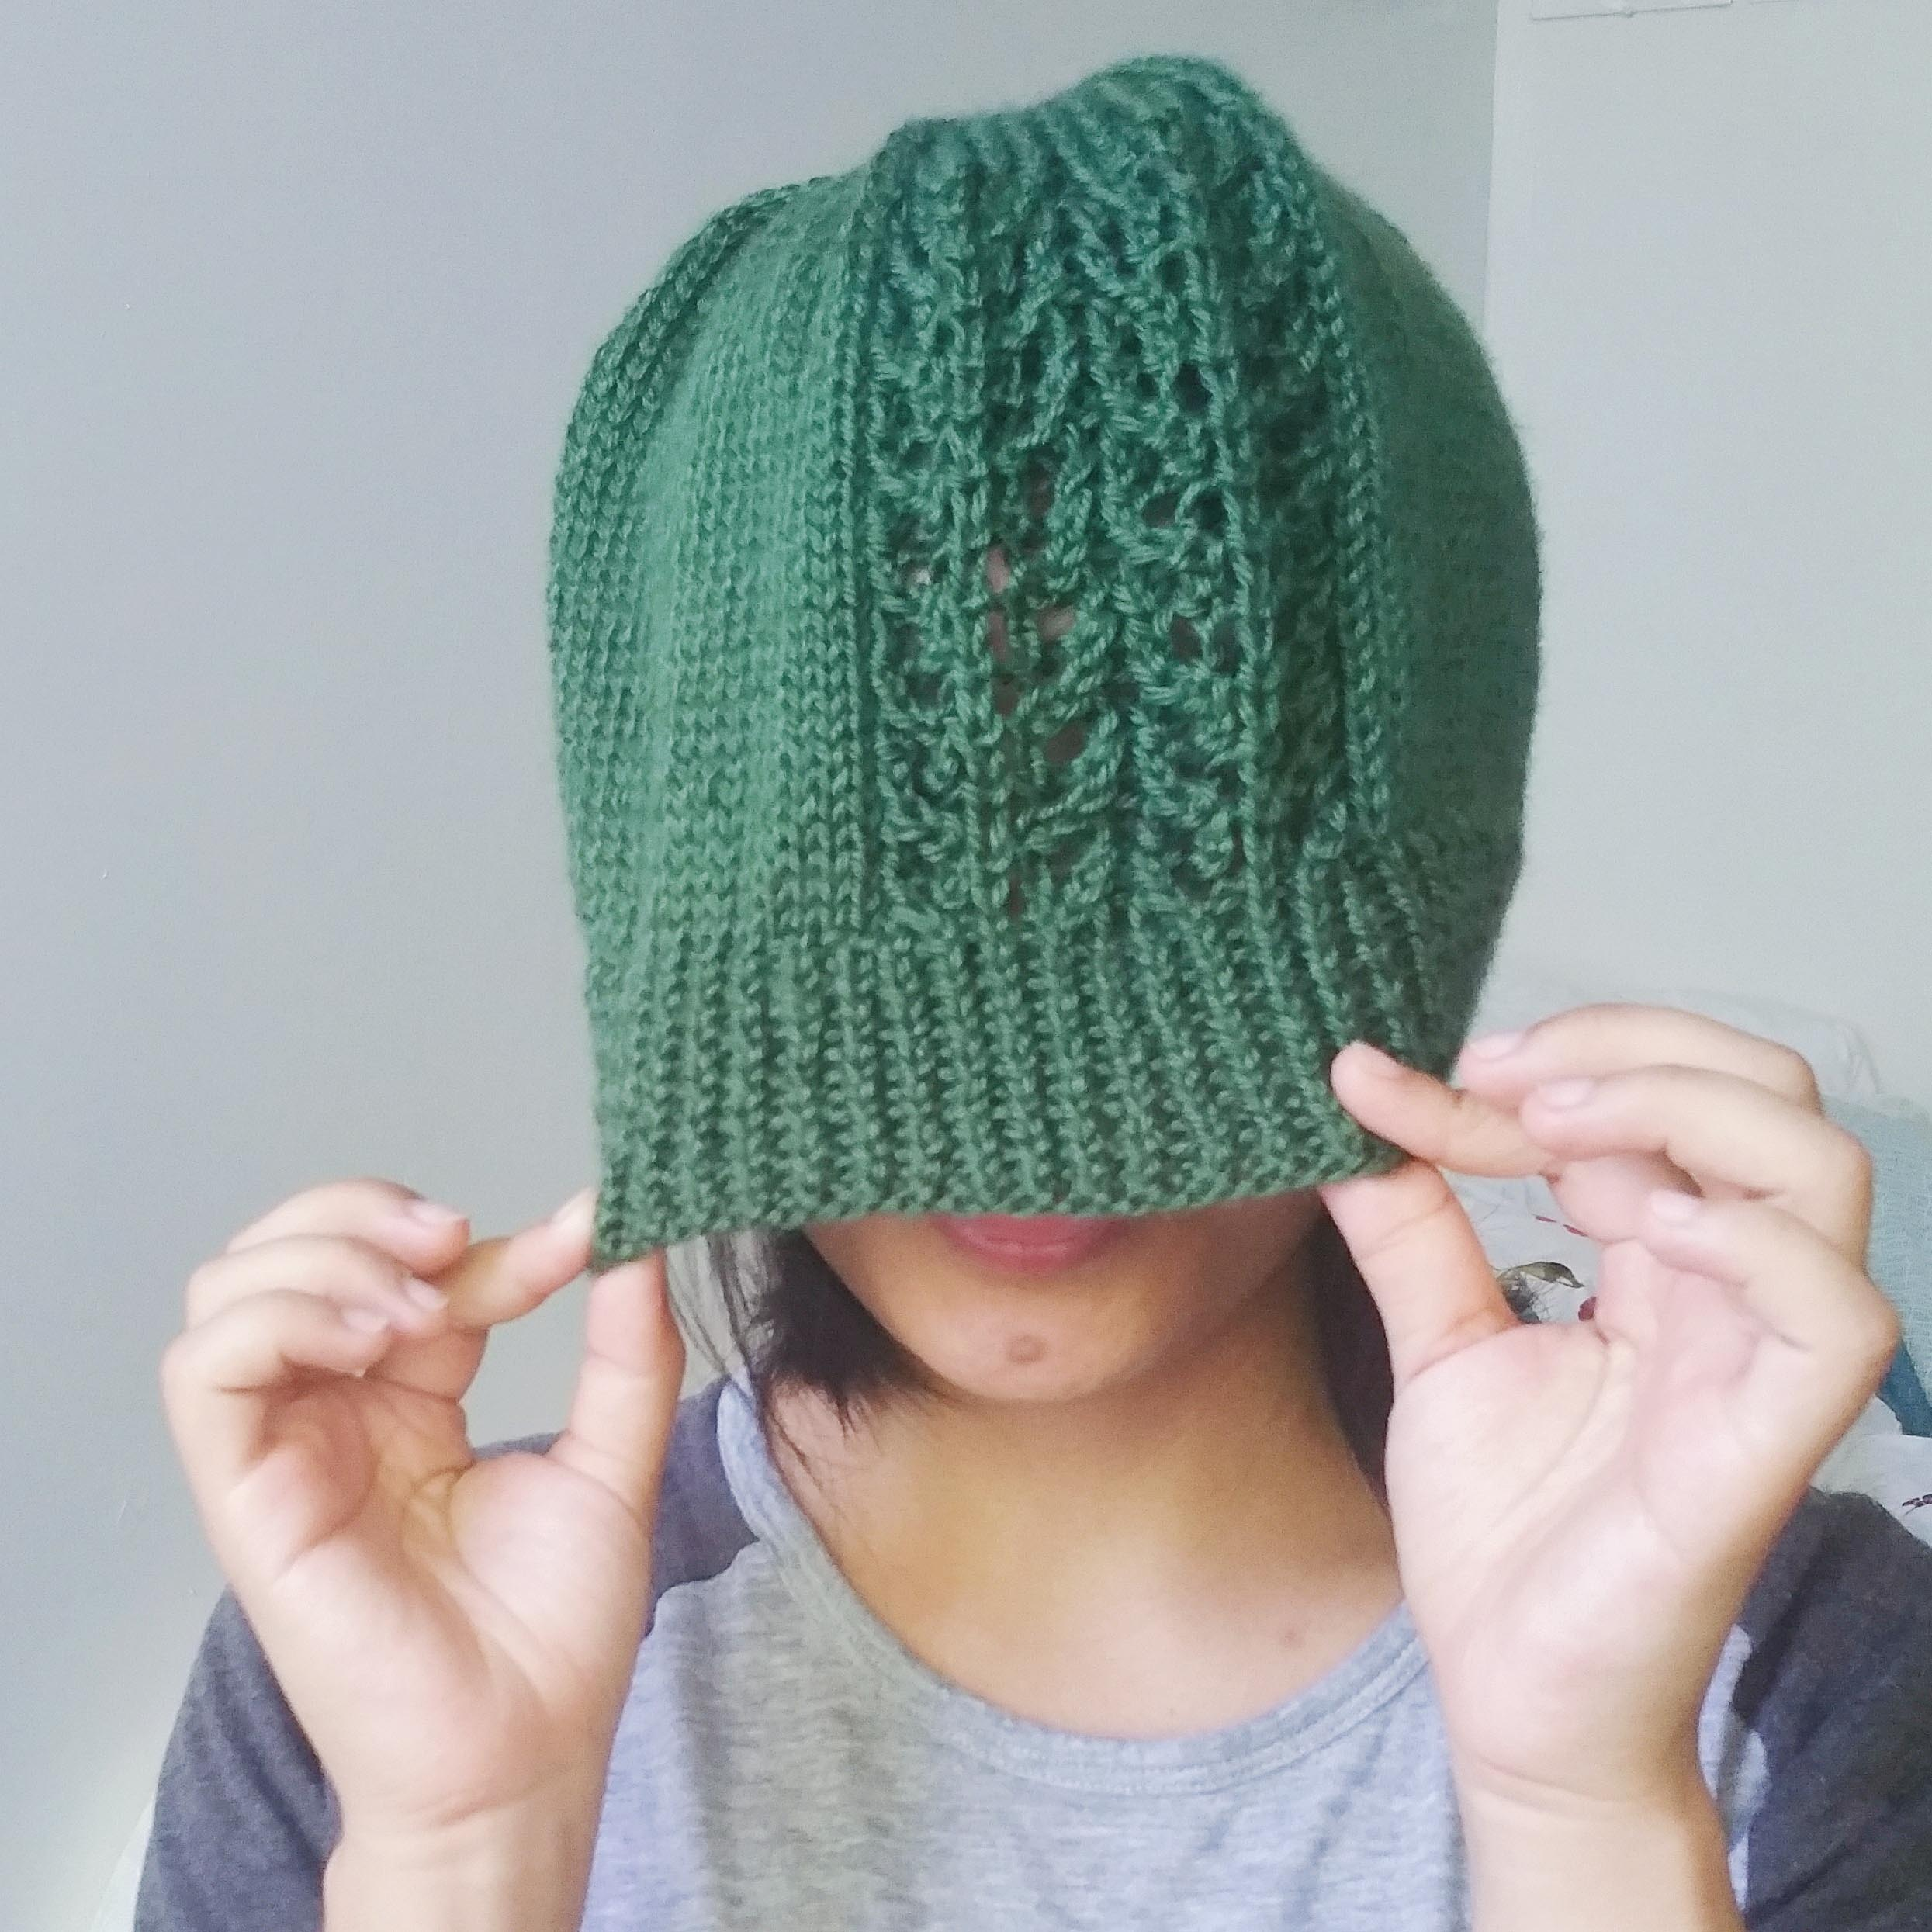
\includegraphics[width=\linewidth]{pullover.jpg}

\section*{\thetitle}
\vspace{-0.5em}
\subsubsection*{\theauthor}

\subsection*{Yarn Requirements}

% 85g/160y worsted weight yarn
% sample: Caron Simply Soft (75g/139y) in "Dark Sage"

100g/190y of worsted weight yarn. Sample used 75g/139y of Caron Simply Soft in ``Dark Sage".

\vspace{-1em}
\subsection*{Tools} \vspace{-.5em}

% US6 for ribbing, US8 for rest
% Sample fits adult head 18" unstretched, 28" stretched
\begin{itemize}
\item 16" circular needle for ribbing \\ (recommended: US6/4.0mm) \vspace{-.5em}
\item 16" circular needle two sizes bigger for hat body (recommended: US8/5.0mm) \vspace{-.5em}
\item DPN set in larger size \vspace{-.5em}
\item tapestry needle\vspace{-.5em}
\item 2-5 stitch markers\vspace{-.5em}
\end{itemize}

\vfill
\columnbreak

\subsection*{Techniques}

This pattern is suitable for an advanced beginner. Prior to knitting this pattern, you must be familiar with knitting in the round, as well as basic lace techniques such as yo, k2tog, and ssk. Instructions for decreases beyond the basics are provided in the pattern key.

\subsection*{Pattern Key}

\vocab{Charts:} repeats = thick borders \chart{\!\underline{\overline{-}}\!}  

\vocab{Written instructions:} 

repeats = \textbf{[stitches]} x \# \emph{or} \textbf{*[stitches]*} to end of round; 
lace section = \highlighted{stitches}
\vspace{-1em}
\begin{center}
{\renewcommand{\arraystretch}{1.5}
\begin{tabular}{| C{0.12\linewidth}  C{0.2\linewidth}  p{0.6\linewidth} | }
\thickhline \rowcolor{shadecolor} 
\textbf{Chart}	& \textbf{Written}	& \textbf{Description} \\ \thickhline
\chart{-}	& k	&  knit \\
\chart{=} 	& p	& purl   \\
\chart{t}	& k tbl	& knit through the back loop \\
\chart{O} 	& yo		& yarn-over  \\
\chart{>}	& k2tog 	& knit 2 together \\
\chart{<}	& ssk		& slip slip knit \\
\chart{R}	& k3tog 	& knit 3 together \\
\chart{L}	& sssk		& \textbf{slip slip slip knit:} slip 3 knitwise individually, k3tog through back loop\\
\chart{A} 	& sk2p	& \textbf{slip k2tog psso} slip 1 st knitwise, k2tog, pass slipped st over (psso)\\
\hline
\end{tabular}
}
\end{center}
\end{multicols}


\subsection*{Sizing/Gauge}

Sample shown stretched over 21" adult head, unblocked. Sample may fit head sizes (plus hair) between 20"-28".
Adjust hat size by changing needle size and/or yarn weight. Hat may grow during blocking.

Gauge (1\x1 ribbing) -- 116 sts/18" = 26sts/4" unstretched,
116 sts/28" = 17 sts/4" stretched. 

\begin{frnote}
\small
\textbf{Modifications:} The following instructions are written for 1 \highlighted{lace panel} and 4 stockinette sections. For 2 lace panels, work \highlighted{lace panel} x 2 then work stockinette sections x 3. For 5 lace panels, work \\\highlighted{lace panel} x 5 to the end of the round without working stockinette.
\end{frnote}


\end{titlingpage}

\begin{multicols}{2}
\section*{1. Ribbing}

With smaller needle, CO 116 sts loosely and join in the round. Place marker (\pm) for the beginning of the round. Work in the following rib pattern until piece measures 2"/5cm, ending after Round~1. Slip marker (\sm) at beginning of round.

\rowDir{Rnd 1} \repeat{k1, p1} 

\rowDir{Rnd 2} \repeat{k1 tbl, p1}

\section*{2. Body}



Switch to larger needle, then work the following set up round: 

\rowDir{Set Up} \sm, \highlighted{k1, p1, \setrepeat{k1 tbl, p1} \x 10, k1,} \highlighted{ {\pm} for end of section,} k to 2 sts from end of round, k2tog. \decrease{1} = \stitchcount{115 total}

\vspace{1em}
For the rest of the body, you will work the lace panel over the 23 sts between the markers, and the rest of the round in stockinette. Work 8 repeats of the lace pattern, or more if you want a longer hat (end after working Rnd 2 or Rnd 4).

\subsection*{Lace (chart)}

\chart{
-\!\overline*{=t=t=t=t=t}\!=- \rnright
-\!=<O<O-O>O>\!=- \rnright
-\!=t=t=t=t=t\!=- \rnright
-\!\underline*{=LO-O-O-OR}\!=- \rnright
}

\vspace{1em}
\chart{-} k \hspace{1em}
\chart{>} k2tog \hspace{1em}
\chart{<} ssk \hspace{1em}
\chart{t} k tbl 

\vspace{.5em}
\chart{=} p \hspace{1em}
\chart{R} k3tog \hspace{1em}
\chart{L} sssk \hspace{1em}
\chart{O} yo


\subsection*{Lace (written)}

\rowDir{Rnd 1} k1, p1, \setrepeat{k3tog, yo, k1, yo, k1, yo, k1, yo, sssk, p1} \x 2, k1

\rowDir{Rnd 2} k1, p1, \setrepeat{k1 tbl, p1} \x 10, k1

\rowDir{Rnd 3} k1, p1, \setrepeat{k2tog, yo, k2tog, yo, k1, yo, ssk, yo, ssk, p1} \x 2, k1

\rowDir{Rnd 4} k1, p1, \setrepeat{k1 tbl, p1} \x 10, k1


\columnbreak

\section*{3. Crown Decreases}

Lace section decreases are highlighted and are also charted. Work 1 set-up round to place additional markers for stockinette sections (if any). Switch to DPN's when appropriate.

\rowDir{Set Up} \sm, \highlighted{\setrepeat{k1, p1} \x 11, k1, } \sm, \\ \repeat{k23, \pm} 4 times to end of round. \stitchcount{115}

\rowDir{Rnd 1} \sm, \highlighted{ssk, \setrepeat{k1 tbl, p1} \x 9, k1 tbl, k2tog,} \repeat{\sm, ssk, k to 2 sts from next marker, k2tog} 4 times to end of round.\\  \decrease{10} = \stitchcount{105 total}.

\rowDir{Rnd 2} \sm, \highlighted{ k2, \setrepeat{p1, k1} \x 9, k1,} \repeat{\sm, k to next marker} 4 times to end of round.

\rowDir{Rnd 3} \sm, \highlighted{k1, \setrepeat{k1 tbl, p1} \x 9, k1 tbl, k1,} work stockinette as in Rnd 2.

\rowDir{Rnd 4} \sm, \highlighted{k2, \setrepeat{p1, k1} \x 9, k1,} work stockinette as in Rnd 2.

\rowDir{Rnd 5} \sm, \highlighted{ssk, \setrepeat{p1, k1 tbl} \x 9, p1, k2tog,} decrease as in Rnd 1.  \decrease{10} = \stitchcount{95 total}.

\rowDir{Rnd 6} \sm, \highlighted{k1, \setrepeat{p1, k1} \x 9,} work stockinette as in Rnd 2.

\rowDir{Rnd 7} \sm, \highlighted{ssk, \setrepeat{k1 tbl, p1} \x 7, k1 tbl, k2tog,} decrease as in Rnd 1. \decrease{10} = \stitchcount{85 total}

\rowDir{Rnd 8} \sm, \highlighted{k2, \setrepeat{p1, k1} \x 7, k1,} work stockinette as in Rnd 2

\rowDir{Rnd 9} \sm, \highlighted{ssk, \setrepeat{p1, k1 tbl} \x 6, p1, k2tog,} decrease as in Rnd 1. \decrease{10} = \stitchcount{75 total}

\rowDir{Rnd 10} \sm, \highlighted{k1, \setrepeat{p1, k1} \x 7,} work stockinette as in Rnd 2.

\rowDir{Rnd 11} \sm, \highlighted{ssk, \setrepeat{k1 tbl, p1} \x 5, k1 tbl, k2tog,} decrease as in Rnd 1. \decrease{10} = \stitchcount{65 total} 

\rowDir{Rnd 12} \sm, \highlighted{k2, \setrepeat{p1, k1} \x 5, k1,} work stockinette as in Rnd 2.

\rowDir{Rnd 13} \sm, \highlighted{ssk, \setrepeat{p1, k1 tbl} \x 4, p1, k2tog,} decrease as in Rnd 1. \decrease{10} = \stitchcount{55 total}

\rowDir{Rnd 14} \sm, \highlighted{ssk, \setrepeat{k1, p1} \x 3, k1, k2tog,} decrease as in Rnd 1. \decrease{10}=\stitchcount{45 total}

\rowDir{Rnd 15} \sm, \highlighted{ssk, p1, k1 tbl, p1, k1 tbl, p1, k2tog,} decrease as in Rnd 1. \decrease{10} = \stitchcount{35 total}

\rowDir{Rnd 16} \sm, \highlighted{ssk, k1, p1, k1, k2tog,} decrease as in Rnd 1. \decrease{10} = \stitchcount{25 total}

\rowDir{Rnd 17} \sm, \highlighted{ssk, p1, k2tog,} decrease as in Rnd 1. \decrease{10} = \stitchcount{15 total}

\rowDir{Rnd 18} \repeat{\rm, sk2p} until all markers removed. \decrease{10} = \stitchcount{5 total}


\subsection*{Lace Section Decreases (chart)}

\chart[right]{
~~~~~~~~~~A~
~~~~~~~~~>=<
~~~~~~~~>-=-<
~~~~~~~>=t=t=<
~~~~~~>-=-=-=-<
~~~~~>=t=t=t=t=<
~~~~--=-=-=-=-=--
~~~~>t=t=t=t=t=t<
~~~-=-=-=-=-=-=-=-
~~~>=t=t=t=t=t=t=<
~~--=-=-=-=-=-=-=--
~~>t=t=t=t=t=t=t=t< 
~-=-=-=-=-=-=-=-=-=- 
~>=t=t=t=t=t=t=t=t=< 
--=-=-=-=-=-=-=-=-=--
-t=t=t=t=t=t=t=t=t=t-
--=-=-=-=-=-=-=-=-=-- 
>t=t=t=t=t=t=t=t=t=t<
}

~\\
~\\
\begin{addmargin}[5em]{0pt}
\setlength{\parskip}{0.5em}
\chart{A} sk2p - s1, k2tog, psso

\chart{<} ssk

\chart{>} k2tog
\end{addmargin}


\end{multicols}
\section*{4. Finishing}

Cut yarn to leave a tail. Using a tapestry needle, draw tail through remaining 5 sts and pull tight to close the hat. Weave in all ends and block if desired. \vspace{1em}

\centering
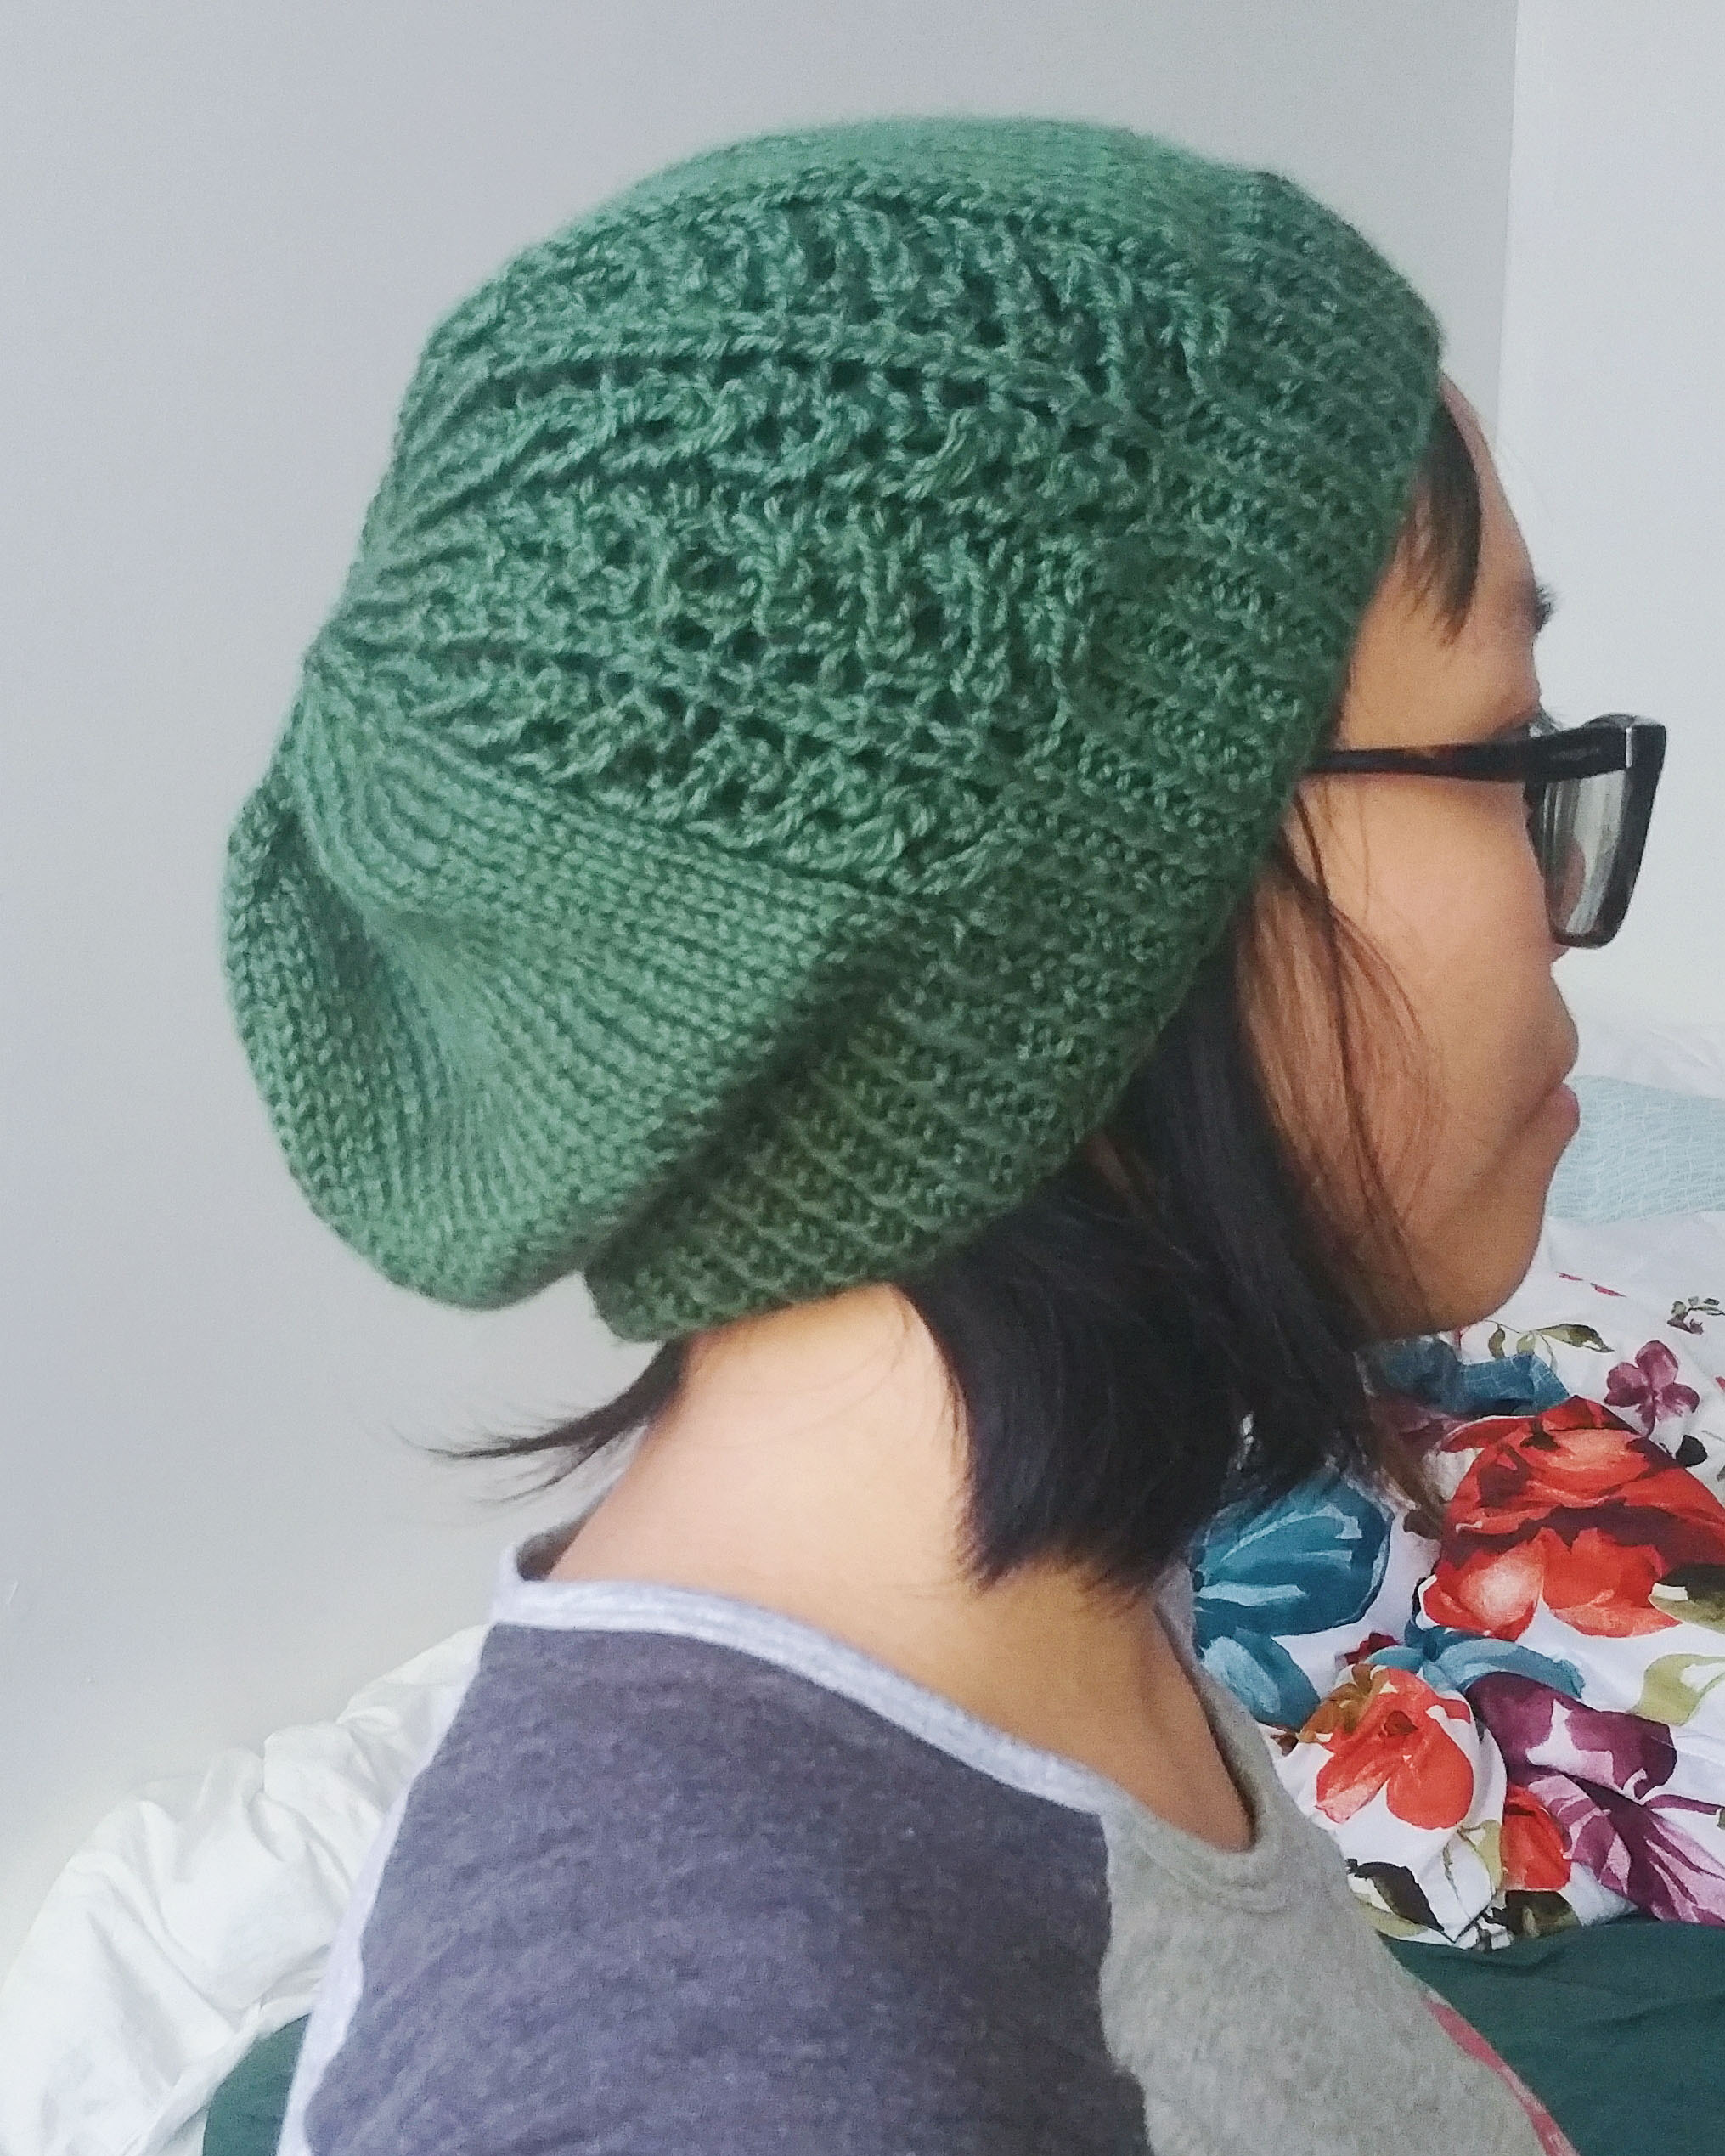
\includegraphics[height=9cm]{sideview.jpg} \hspace{1em}
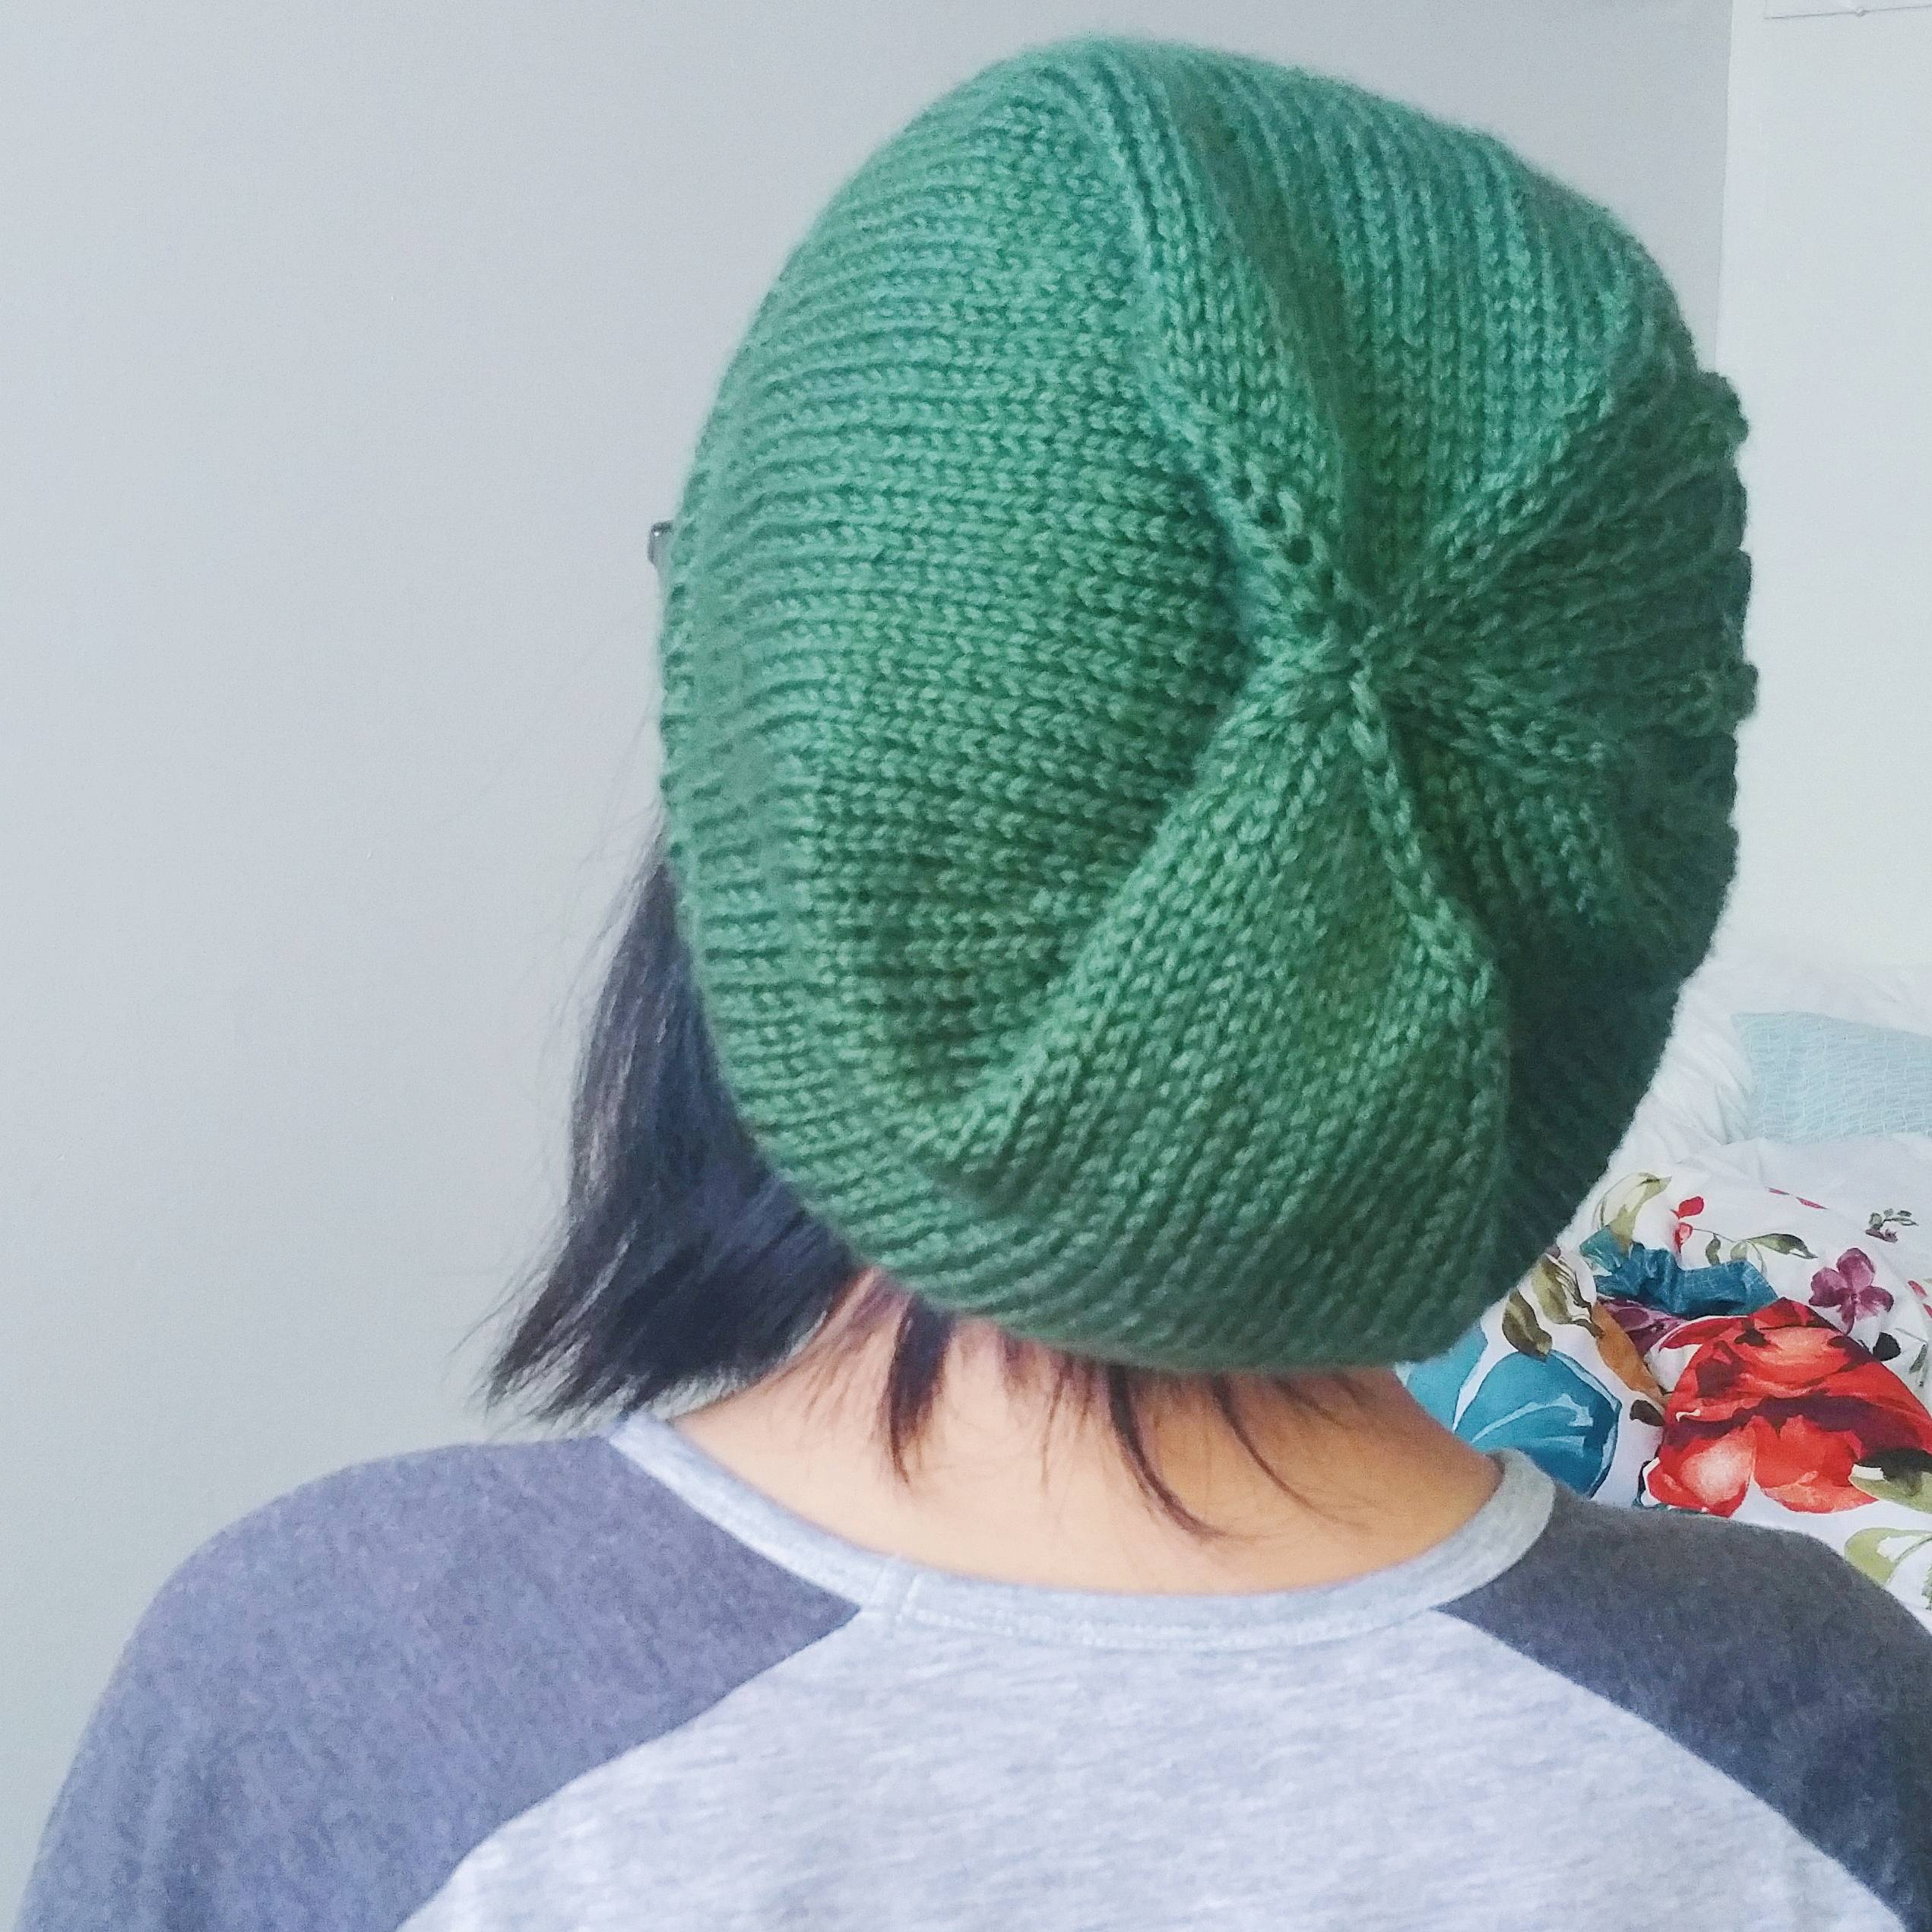
\includegraphics[height=9cm]{decreases.jpg}
\end{document}